
\appendix
\renewcommand{\chaptermark}[1]{\markboth{Appendix \thechapter\relax:\thinspace\relax#1}{}}
\com{
\chapter{Model of the sensors}


\section{Kinematic Model}
\noindent
$$
  \label{eq:state}
\mathbf{X}_t=
\begin{bmatrix}
\mathbf{x}_t \\ \mathbf{y}_t \\ \boldsymbol \theta_t \\ \mathbf{v}_t \\ \boldsymbol \omega_t \\ \mathbf{a}_t \\[0.3em]
\end{bmatrix}
$$

\begin{equation}
A_t
=
\begin{bmatrix}
1 & 0 & 0 & dt \cdot \cos(\boldsymbol \theta_t) & 0 & \frac{dt^2 \cdot \cos(\boldsymbol \theta_t)}{2} \\
0 & 1 & 0 & dt \cdot \sin(\boldsymbol \theta_t)& 0 & \frac{dt^2 \cdot \sin(\boldsymbol \theta_t)}{2} \\
0 & 0 & 1 & 0 & dt & 0 \\
0 & 0 & 0 & 1 & 0 & dt \\
0 & 0 & 0 & 0 & 1 & 0 \\
0 & 0 & 0 & 0 & 0 & 1 \\[0.3em]
\end{bmatrix}
\end{equation}

\begin{equation}
    \mathbf{X}_t = A \cdot \mathbf{X}_{t-1}
\end{equation}

\section{Wheel Encoder information}

$$
Wheel~meter~per~tick = \frac{( 2 \cdot \pi ) \cdot ( \frac{Wheel~diameter}{2}) }{Wheel~Pulses~per~turn}
$$


$$
\Delta _{PulsesRight} = Right~Pulses - Previous~Right~Pulses
$$
$$
\Delta _{PulsesLeft}  = Left~Pulses  - Previous~Left~Pulses
$$


$$
\Delta _{Right} ~ = \Delta _{PulsesRight} \cdot Wheel~meter~per~tick
$$
$$
\Delta _{Left} ~ = \Delta _{PulsesLeft} \cdot Wheel~meter~per~tick
$$

$$
\Delta s = \frac{\Delta _{Right} + \Delta _{Left}}{2}
$$


$$
\Delta {\theta} = \frac{\Delta _{Right} - \Delta _{Left}}{Base~Width}
$$

\subsection{Euler Encoder Model}

\noindent This is the integration method adopted. It is a precise enough approximation of the
$$
x_{t+1} = x_t + \Delta s \cdot \cos(\theta_t)
$$
$$
y_{t+1} = y_t + \Delta s \cdot \sin(\theta_t)
$$
$$
\theta_{t+1} = \theta_t + \Delta {\theta}
$$

\subsection{Runge-Kutta 2 Encoder Model}

\noindent It is supposed to be slightly more precise, but since the improvements at such an high frequency are non relevant then it is not considered.
$$
x_{t+1} = x_t + \Delta s \cdot \cos(\theta_t + \frac{\Delta{\theta}}{2} )
$$
$$
y_{t+1} = y_t + \Delta s \cdot \sin(\theta_t + \frac{\Delta{\theta}}{2} )
$$
$$
\theta_{t+1} = \theta_t + \Delta {\theta}
$$





\section{GPS}
\noindent
From geodetic coordinates to ENU coordinates, as specified by ROS REP 103 and 105.

Using \com{the tool pymap3d\footnote{https://github.com/geospace-code/pymap3d} or} specific math equations derived by Vincenty solutions of geodesics on the ellipsoid\footnote{Vincenty's formulae  -  Direct and Inverse solutions of geodesics on the ellipsoid with application of nested equations}, through the function geodetic2enu that computest the difference between the initial gps average position of the base station and the current reading obtained by the GPS receiver.

First a translation from the geodetic coordinates in WSG-84 degrees estimated by the GPS receiver sensors to the ECEF coordinates is implemented, it is done so both for the initial coordinate and then used to check the difference with the ECEF translation from the geodetic coordinates of the successive reading of the GPS receiver.


%GPS positioning is in the global coordinate system WGS84 [18].

From World Geodetic System: WGS 84 values
\begin{align}
    EqR &= 6378137 && \text{Equatorial radius (m)} \\
    PoR &= 6356752.3142 && \text{Polar radius (m)}
\end{align}

From which the following can be derived the following values necessary for the next algorithms:
\begin{align}
    f &= \frac{EqR - PoR}{EqR} \\
    e\_sq &= f \cdot (2-f)
\end{align}

Using these values it is possible to transform from Geodetic WSG-84 Coordinates to ECEF coordinates using the  Algorithm specified in \ref{alg:ecef}.


\begin{algorithm}[H]
\caption{Geodetic to ECEF Coordinates }
\label{alg:ecefApp}
  \hspace*{\algorithmicindent} \textbf{Input:} Latitude and Longitude ($lat$, $lon$) in WSG-84 degrees\\
  \hspace*{4em} Altitude ($h$) in meters\\
  \hspace*{\algorithmicindent} \textbf{Output:} ECEF Coordinates in meters ($x$, $y$, $z$)
  %\KwData{Testing set $x$}
  %$\sum_{i=1}^{\infty} := 0$ \tcp*{this is a comment}
  %\tcc{Transform latitude and longitude}
  \begin{algorithmic}[1]
  \STATE $N = \cfrac{EqR}{\sqrt{1 - e\_sq \cdot \sin(lat)^2}}$
  \STATE $x = (h + N) \cdot \sin(lat) \cdot \cos(lon)$
  \STATE $y = (h + N) \cdot \cos(lat) \cdot \sin(lon)$
  \STATE $z = (h + (1 - e\_sq) \cdot N) \cdot \sin(lat)$
  \STATE return $x$, $y$, $z$
    \end{algorithmic}
\end{algorithm}

Finally, by exploiting the previous algorithm, it is possible to transform the Current Geodetic Coordinates into Local Coordinates by using some Reference Geodetic Coordinates and the following Algorithm \ref{alg:local}.

\begin{algorithm}[H]
\caption{Geodetic to Local using Current and Reference Coordinates}
\label{alg:localApp}
    \hspace*{\algorithmicindent} \textbf{Input:} Current Latitude and Longitude ($latC$, $lonC$)\\
        \hspace*{5em} in WSG-84 degrees\\
    \hspace*{4em} Current Altitude ($hC$) in meters\\
    \hspace*{4em} Reference Latitude and Longitude ($latR$, $lonR$)\\
        \hspace*{5em} in WSG-84 degrees\\
    \hspace*{4em} Reference Altitude ($hR$) in meters \\
    \hspace*{\algorithmicindent} \textbf{Output:} Local Coordinates in meters ($\Delta x$, $\Delta y$, $\Delta z$)
  \begin{algorithmic}[1]
    \STATE $xC$, $yC$, $zC$ = Geodetic to ECEF Coordinates ($latC$, $lonC$, $hC$)
    \STATE $xR$, $yR$, $zR$ = Geodetic to ECEF Coordinates ($latR$, $lonR$, $hR$)
    \STATE $xD = xC - xR$
    \STATE $yD = yC - yR$
    \STATE $zD = zC - zR$
    \STATE $\Delta x = -~\sin(lonR)~\cdot~xD~+~\cos(latR)~\cdot~yD$
    \STATE $\Delta y = -~cos(lonR)~\cdot~\sin(latR)~\cdot~xD~-~\sin(latR)~\cdot~\sin(lonR)~\cdot~yD~+ \hspace*{3em} \cos(latR)~\cdot~zD$
    \STATE $\Delta z = \cos(latR)~\cdot~\cos(lonR)~\cdot~xD~+~\cos(latR)~\cdot~\sin(lonR)~\cdot~yD~+  \hspace*{3em} \sin(latR)~\cdot~zD$
    \STATE return $\Delta x$, $\Delta y$, $\Delta z$
    \end{algorithmic}

\end{algorithm}

\com{
\begin{figure}
	\begin{center}
		%\includegraphics{Images/4-Methods/Figure_2.png.eps}
		%\includesvg{Images/4-Methods/Figure_2.png.svg}
		%\input{Images/4-Methods/Original-Fig-GPSfix.pgf}
	\end{center}
	\caption{A PGF histogram from \texttt{matplotlib}.}
\end{figure}
}

\section{IMU}

\noindent
As IMU sensor we use the PhidgetSpatial Precision 3/3/3 High Resolution \footnote{https://www.phidgets.com/?tier=3\&catid=10\&pcid=8\&prodid=1158}.
We use its APIs to gather the measurements and then publish them as ROS topics, after some tunings.

\section{Camera}

\noindent The camera is the Intel RealSense D435 and the \gls{VO} package is \gls{RTABMAP}.

}



\chapter{Competitor Analysis}

\noindent As this master thesis has been developed under the programme of EIT Digital\footnote{\url{https://masterschool.eitdigital.eu/}}, an analysis of the competitor will be performed to highlight the current state of the art at an industrial level for \glspl{ALM} which require no boundary wire installation, understanding their current implementations, and evaluating possible improvements.

Toadi\footnote{\url{https://www.toadi.com/}} is a startup company based in Belgium which offers as only product an \gls{ALM} of the same name. It employs a single visual sensor system to provide the localisation features. It can mow an area of \SI{4800}{\meter\squared}.
Its installation is performed though a track and follow approach to determine the boundaries of the lawn, it has been in testing phase and it is available to the public from May 2021.

The LUNA platform from Inertial Systems\footnote{\url{https://inertialsense.com/autonomy/}} employs all the sensors listed above to provide a localisation and navigation module, which has been used for \glspl{ALM}. This platform was developed to enable engineers to directly embed autonomous capability into existing equipment avoiding the development of a localisation module, as it is detailed in this thesis.

Kingdom Technologies\footnote{\url{https://www.kingdom.garden/}} provide an \gls{ALM} at a monthly fee to commercial clients.
It employs sensor fusion techniques to merge several different sensors' measures to improve the positioning of the robot on a lawn that could reach an area of \SI{7500}{\meter\squared}.

Ambrogio L60 Elite S+\footnote{\url{https://www.ambrogiorobot.com/en/models/view/l60-elite-s}} requires no installation for areas up to \SI{400}{\meter\squared}.
It employs a grass sensor to detect the presence of grass under itself and it uses a specific robotic joint to recognise any holes or empty spaces. With these sensors it is able to navigate around a defined lawn using a reactive approach, but without the need for the boundary wire.

Different approaches which do not require the boundary wire installation but which still need some external infrastructures are the following.

Husvarna 550 EPOS\footnote{\url{https://www.husqvarna.com/us/products/robotic-lawn-mowers/models/automower-550-epos/}} is a new \gls{ALM} available for commercial customers which employs a \gls{GPSRTK} sensor to cover areas of \SI{5000}{\meter\squared}. It needs an external and expensive receiver to correct the \gls{GNSS} estimates of the robot and improve its localisation performance to just a few centimeters error.

iRobot Terra t7\footnote{\url{https://www.irobot.co.uk/Terra}} is the \gls{ALM}
It relies on wireless navigation beacons installed on the garden to triangulate the position of the mower using their signals. However, the implementation of such technology has concerned the \gls{NRAO}, as the original intended frequency they used were disturbing the measurements of that organisation, and they had to change their beacons using \gls{UWB} signal technology.

The currently developed \glspl{ALM} are still far from being mature and available to all customers.
For this reason, an analysis of the best configuration of sensors to improve on the localisation aspects without the need for an external installation is provided, as improved localisation performance of autonomous mobile robots are required.

Numerous related studies and implementations have been developed in similar topics to improve localisation features, and the analysis of an optimal configuration of sensors which require no external installations is still relevant to the best of the found knowledge.



\chapter{Highly-Non-Linear Sensor Fusion}
\noindent The system analysed in this thesis is not characterised by high non-linearity given the high frame-rate available, and as such the adopted \gls{AEKF} is robust, fast, and sufficient.

A brief description of other linearisations, such as the \gls{UKF}, and other approaches, such as \gls{PF}, are provided in this appendix.
Even if they are not used in this thesis, they are noteworthy to mention to provide a more comprehensive overview of sensor fusion techniques, in case of highly non linear systems.

\section{Unscented Kalman Filter}
\label{sec:ukf}
\noindent The \gls{UKF} is an alternative to the \gls{KF} for estimation of highly non linear systems~\cite{unscentedK}.
Instead of using a linearisation approach, the \gls{UKF} is based on a deterministic sampling method.
The estimates are propagated through the non linear system using sample values, called sigma points, defined by the unscented transform.
This procedure provides two values along the mean of the estimate and symmetrically placed on its main uncertainty axes.
Although the results are not a Gaussian random variables, their mean and standard deviation can be derived from them to maintain the \gls{KF} assumption.

Its improvements in estimates and covariance accuracy are relevant over the \gls{EKF} when the functions $f$ and $h$ are highly non-linear, as it is accurate to the second order Taylor's expansion.
Moreover, it does not need to compute Jacobians of the non linear functions of the system~\cite{thrun_probabilistic_2005}.



\section{Particle Filter}
\label{sec:pf}
\noindent The \gls{PF} provides another implementation of a Bayesian filter~\cite{particle}.
It is an iterative algorithm which saves multiple potential state estimate values, known as particles.
The probability the state estimate value in a moment in time is given by the density of particles nearby which contains similar values.
At each iteration, a sampling phase is performed generating temporary particles using the current estimated state.
Afterwards an importance factor is calculated using new measurements of the state and it provides a likelihood value for the next estimations.
In the resampling phase, the proper particles are updated by using the estimates provided by one of the temporary particles with a selection based on the importance factor.
This process is continuously iterate and the particles will eventually converge to a proper estimate over several steps.

The Rao-Blackwellized \gls{PF} extends it using both particles and Gaussian random variables as state variables~\cite{murphy_rao-blackwellised_2001}.




\chapter{Robotic Operating System}
\label{ch:ros}
\noindent \Gls{ROS}\cite{288} is an open-source framework, and not an actual operating system, widely adopted for building software used to control robotic systems.
\Gls{ROS} works both with C++ and Python programmed scripts, allowing for developers with different backgrounds to develop upon it.


For these nodes to cooperate, they are connected by a middle-layer structure based on a network of topics or services, following a blackboard architecture of data sharing.
It provides a graph-like structure were each program, described as node, can both publish and subscribe messages among the created and available topics.

Topics can be seen as variables which are used for streaming communication and share information between nodes.
A \Gls{ROS} node publishes a specific message through a topic and every other node can subscribe to that topic and receive all the messages posted to it.
A \Gls{ROS} system, to behave as expected, needs a master process which has the task of matching publishers and subscribers to their related topics.

These topics can be generated by sensors, actuators, planners, controllers of different kind and made available using this structure of topics, similar to a blackboard architecture.
Each topic is defined by a specific message type which specifies its content in order to standardise its usage among applications and to simplify communication between nodes.
Messages definition can be customised and they are stored inside the \Gls{ROS} package, defining the data sent within the topic which will use that definition.

Figure \ref{fig:ros-topic} shows an example of a \Gls{ROS} graph where two subscriber nodes receive the messages posted on the topic by a publisher node.

\begin{figure}[!ht]
	%\textbf{Investigating Simultaneous Localization and Mapping for AGV systems}
	\begin{center}
		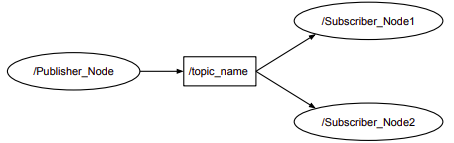
\includegraphics[width=0.75\textwidth]{Images/2-Background/ROSTopic-2021-04-22 10-51-37.png}
	\end{center}
	\caption{\Gls{ROS} topics architecture}% for information sharing\cite{palsson_investigating_2017}}
	\label{fig:ros-topic}
\end{figure}

The aspect of localisation is important for the robotics field, to understand where the robot is located with respect to the rest of the world, but also to know how the sensors are positioned with respect to the robot in which they are installed.
It is of prominent importance to be aware of the different pose of the connected sensors before fusing their information, as the measurements of each sensors are related to their specific coordinate frame.

Before performing sensors fusion, every different frames of the sensors need to be transformed into the base frame of the robot which they are measuring to be sure about that the measurements refers to the same coordinate frame.

\Gls{ROS} uses the TF\cite{6556373} library to provide the tools needed to work with coordinate frames and to deal with their related transformation.
It allows for the definition of each sensor rigid body transform to specify their related position with respect to the robot, and then the library will deal with all the other transformations by publishing messages regarding to the rotational and translational relations between frames.
Commonly used frames are odom and base\_link. The odom frame has the origin at the initial position $P_{odom}$ of the robot and it is used to keep track of its moving behaviour. The base\_link frame is rigidly attached to the robot base $P_{base}$ and it is used to define the frames of its attached components.

\begin{figure}[!ht]
	%\textbf{Investigating Simultaneous Localization and Mapping for AGV systems}
	\begin{center}
		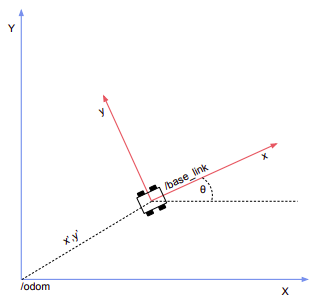
\includegraphics[width=0.75\textwidth]{Images/2-Background/Frames-2021-04-22 12-03-22.png}
	\end{center}
	\caption{\Gls{ROS} frames architecture}% for information sharing\cite{palsson_investigating_2017}}
	\label{fig:ros-frame}
\end{figure}



\chapter{Repository}
\noindent
Everything that has been developed during this thesis could be found in \url{https://github.com/boffomarco/hrp}

The following files are the main contributions provide in this thesis.

\section{System Configuration}
\noindent


.bashrc

network\_file \todo{Configuration of network settings between RPis and PC using ROS to be added in a file describing the procedure}

\section{Localisation Configuration}
\noindent The improved localisation performance are provided using a personalised configuration of the sensors and the related sensor fusion of their measures.

sensors.launch

automower\_safe.launch

imus\_basic.launch

gps.launch

gps.cpp

rs\_camera.launch

rtabmap.launch

BatchEKF.launch

BatchEKF\_last.py

BatchEKF\_lastRPi.py

BatchEKF\_lastSimulated.py

GroundTruthSimulated.py

\section{Mapping Configuration}
\noindent

OccupancyGrid.py

\section{Results Configuration}
\noindent

plot\_histogram.py

gps\_plot.py



%\chapter{Something Extra}
